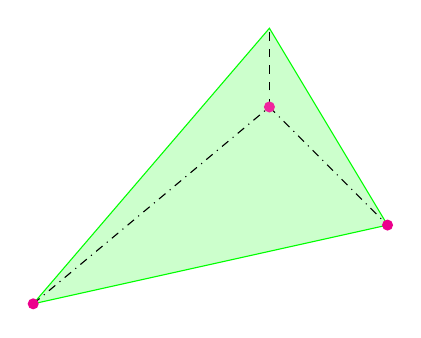
\begin{tikzpicture}	
	\coordinate (A) at (0,0);
	\coordinate (B) at (3,2.5); % pivot
	\coordinate (C) at (4.5,1);

	\coordinate (T) at (3,3.5);	
	
	\fill[green!20] (A)--(T)--(C)--(A);
	\draw[green] (A)--(T)--(C)--(A);
	\draw[dash dot] (A)--(B)--(C);
	\draw[dashed] (B)--(T);
	
	\foreach \p in {(A),(C)}	
		\fill[magenta] \p circle (2pt);
	\fill[magenta!85] (B) circle (2pt);
\end{tikzpicture}